
\section{Type 1 combinatorial Reeb orbits}
\label{sec:type1}

Let $X$ be a symplectic polytope in $\R^4$. In this section we give what amounts to an algorithm for finding the Type 1 combinatorial Reeb orbits and their combinatorial symplectic actions, see Proposition~\ref{prop:orbitbijection}. (Our actual computer implementation uses various optimizations not discussed here.) We also define combinatorial rotation numbers and work out the example of the 24-cell.

\subsection{Symplectic flow graphs}
\label{subsec:symplectic_flow_graphs}

We start by defining ``symplectic flow graphs'' in any even dimension. In the next subsection (\S \ref{subsubsec:symplectic_polytopes}), we will specialize to certain $2$-dimensional flow graphs that keep track of the combinatorics needed to find Type 1 Reeb orbits on the boundary of a symplectic polytope in $\R^4$. 

\begin{definition}
\label{def:linear_domain}
A {\bf linear domain\/} is an intersection of a finite number of open or closed half-spaces in an affine space, or an affine space itself.
\end{definition}

\begin{definition}
\label{def:tangent_space} The {\bf tangent space} $TA$ of a linear domain $A$ is the tangent space $T_xA$ for any $x\in A$; the tangent spaces for different $x$ are canonically isomorphic to each other via translations.
\end{definition}

\begin{definition}
\label{def:affine_map_of_linear_domains}
Let $A$ and $B$ be linear domains. An {\bf affine map} $\phi:A \to B$ is the restriction of an affine map between affine spaces containing $A$ and $B$. Such a map induces a map on tangent spaces which we denote by $T\phi: TA\to TB$.
\end{definition}

\begin{definition}
\label{def:linear_flow}
Let $A$ and $B$ be linear domains. A {\bf linear flow} from $A$ to $B$ is a triple $\Phi = (D,\phi,f)$ consisting of:
\begin{itemize}
	\item the {\bf domain of definition}: a linear domain $D \subset A$.
	\item the {\bf flow map}: an affine map $\phi:D \to B$.
	\item the {\bf action function}: an affine function $f:D \to \R$.
\end{itemize}
We sometimes write $\Phi:A\to B$. In the examples of interest for us, $\phi$ is injective, and $f\ge 0$.
\end{definition}

\begin{definition}
\label{def:linear_flow_composition}
Let $\Phi = (D,\phi,f)$ be a linear flow from $A$ to $B$ and let $\Psi = (E,\psi,g)$ be a linear flow from $B$ to $C$. Their {\bf composition} is the linear flow $\Psi \circ \Phi: A \to C$ defined by
\[
\Psi \circ \Phi = (\phi^{-1}(E),\psi \circ \phi, f + g \circ \phi).
\]
\end{definition}

\begin{remark} Composition of linear flows is associative, and there is an identity linear flow $\iota_A:A \to A$ given by $\iota_A = (A,\op{id}_A,0)$. If $\Phi_i=(D_i,\phi_i,f_i)$ is a linear flow from $A_{i-1}$ to $A_i$ for $i=1,\ldots,k$, and if $\Phi=(D,\phi,f)$ is the composition $\Phi_k\circ\cdots\circ \Phi_1$, then for $x\in D$, we have
\begin{equation}
\label{eqn:actioncomposition}
f(x) = \sum_{i=1}^kf_i((\phi_{i-1}\circ\cdots\circ\phi_1)(x)).
\end{equation}
\end{remark}

\begin{definition}
\label{def:linear_flow_graph}
A {\bf linear flow graph} $G$ is a triple $G = (\Gamma,A,\Phi)$ consisting of:
\begin{itemize}
 \item A directed graph $\Gamma$ with vertex set $V(\Gamma)$ and edge set $E(\Gamma)$.
 \item For each vertex $v$ of $\Gamma$, an open linear domain $A_v$.
 \item For each edge $e$ of $\Gamma$ from $u$ to $v$, a linear flow $\Phi_e = (D_e,\phi_e,f_e):A_u \to A_v$.
\end{itemize}
\end{definition}

\begin{figure}[h!]
\label{fig:flow_graph}
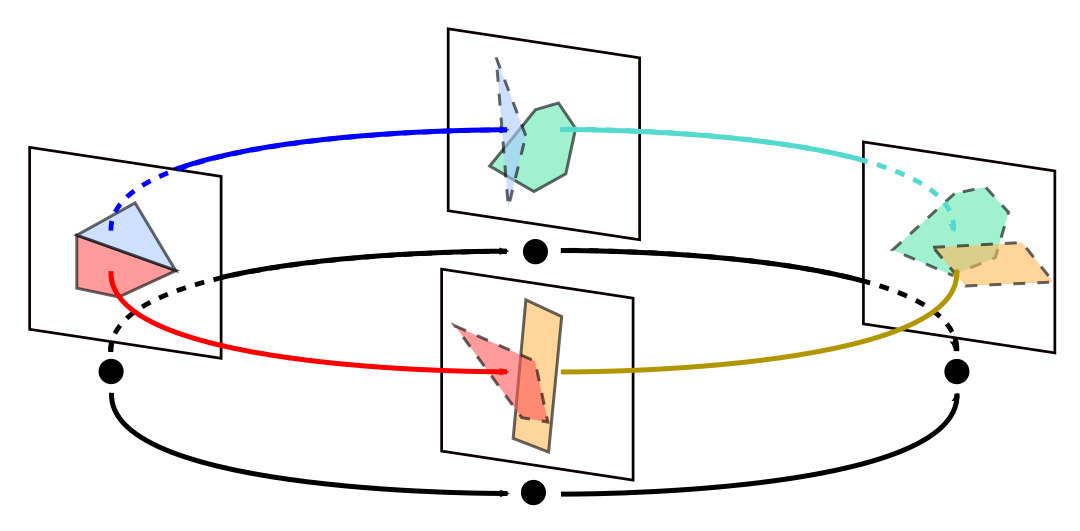
\includegraphics[width=\linewidth]{flow_graph.png}
\caption{An example of a flow graph with 4 nodes and 4 edges. The linear domains and flows are depicted above their corresponding nodes and edges.}
\end{figure}

Let $G=(\Gamma,A,\Phi)$ be a linear flow graph. If $p = e_1\dots e_k$ is a path in $\Gamma$ from $u$ to $v$, we define an associated linear flow
\[
\Phi_p = (D_p,\phi_p,f_p) : A_u \longrightarrow A_v
\]
by
\[
\Phi_p = \Phi_{e_k} \circ \dots \circ \Phi_{e_1}.
\]

\begin{definition}
\label{def:flow_graph_trajectory}
A {\bf trajectory} $\gamma$ of $G$ is a pair $\gamma = (p,x)$, where $p$ is a path in $\Gamma$ and $x \in D_p$.
\end{definition}

\begin{definition}
\label{def:flow_graph_periodic_orbit}
A {\bf periodic orbit} of $G$ is an equivalence class of trajectories $\gamma = (p,x)$ where $p$ is a cycle in $\Gamma$ and $x$ is a fixed point of $\phi_p$, i.e.\ $\phi_p(x) = x$. Two such trajectories $\gamma = (p,x)$ and $\eta = (q,y)$ are equivalent if there are paths $r$ and $s$ in $\Gamma$ such that $p = rs$, $q = sr$, and $\phi_r(x) = y$. We often abuse notation and denote the periodic orbit by $\gamma=(p,x)$, instead of by the equivalence class thereof.
\end{definition}

\begin{definition}
\label{def:action_of_periodic_orbit}
The {\bf action} of a periodic orbit $\gamma = (p,x)$ is defined by $f(\gamma) = f_p(x)$.
\end{definition}

\begin{definition} \label{def:degenerate_orbit} A periodic orbit $\gamma = (p,x)$, where $p$ is a cycle based at $u$, is {\bf degenerate} if the induced map on tangent spaces $T\phi_p:TD_u \to TD_u$ has $1$ as an eigenvalue. Otherwise we say that $\gamma$ is {\bf nondegenerate\/}.
\end{definition}

\begin{definition}
\label{def:symplectic_flow_graph}
An $2n$-dimensional {\bf symplectic flow graph\/} $G$ is a quadruple $G = (\Gamma,A,\omega,\Phi)$ where:
\begin{itemize}
	\item $(\Gamma,A,\Phi)$ is a linear flow graph in which each linear domain $A_v$ has dimension $2n$.
	\item $\omega$ assigns to each vertex $v$ of $\Gamma$ a linear symplectic form $\omega_v$ on $TA_v$.
  \end{itemize}
We require that if $e$ is an edge from $u$ to $v$, then $\phi_e^*\omega_v = \omega_u$.
\end{definition}

\subsection{The symplectic flow graph of a 4d symplectic polytope}
\label{subsubsec:symplectic_polytopes}

\begin{definition}
\label{def:sfgp}
Let $X$ be a symplectic polytope in $\R^4$. We associate to $X$ the two-dimensional symplectic flow graph $G(X)=(\Gamma,A,\omega,\Phi)$ defined as follows:
\begin{itemize}
    \item The vertex set of $\Gamma$ is the set of $2$-faces of $X$. The linear domain associated to a vertex is simply the corresponding $2$-face, regarded as a linear domain in $\R^4$. If $F$ is a $2$-face, then the symplectic form $\omega_F$ on $TF$ is the restriction of the standard symplectic form $\omega_0$ on $\R^4$.
    \item If $F_1$ and $F_2$ are $2$-faces, then there is an edge $e$ in $\Gamma$ from $F_1$ to $F_2$ if and only if there is a $3$-face $E$ adjacent to $F_1$ and $F_2$, and a trajectory of the Reeb vector field $R_E$ on $E$ from some point in $F_1$ to some point in $F_2$. In this case, the linear flow
    \[
\Phi_e = (D_e,\phi_e,f_e):F_1\longrightarrow F_2
    \]
    is defined as follows:
\begin{itemize}
  \item
  The domain $D_e$ is the set of $x\in F_1$ such that there exists a trajectory of $R_E$ from $x$ to some point $y\in F_2$.
  \item
  For $x$ as above, $\phi_e(x)=y$, and $f_e(x)$ is the time it takes to flow along the vector field $R_E$ from $x$ to $y$, or equivalently the integral of $\lambda_0$ along the line segment from $x$ to $y$.
 \end{itemize}
\end{itemize} 
\end{definition}

In the above definition, note that $\phi_e$ and $f_e$ are affine, because the vector field $R_E$ on $E$ is constant by equation \eqref{eqn:Reebinu}.  A simple calculation as in \cite[Eq.\ (5.10)]{hwz} shows that the map $\phi_e$ is symplectic.

\begin{proposition}
\label{prop:orbitbijection}
Let $X$ be a symplectic polytope in $\R^4$. Then there is a canonical bijection
\[
\{\mbox{periodic orbits of $G(X)$}\} \longleftrightarrow \{\mbox{Type $1$ combinatorial Reeb orbits of $X$}\}.
\]
If $(p,x)$ is a periodic orbit of $G(X)$, and if $\gamma$ is the corresponding combinatorial Reeb orbit, then
\begin{equation}
\label{eqn:identifyactions}
f(p,x) = \mc{A}_{\op{comb}}(\gamma).
\end{equation}
\end{proposition}

\begin{proof}
Suppose $(p=e_1\cdots e_k,x)$ is a periodic orbit of $G(X)$. Let $E_i$ denote the $3$-face of $X$ associated to $e_i$. There is then a combinatorial Reeb orbit $\gamma=(L_1,\ldots,L_k)$, where $L_i$ is the line segment in $E_i$ from $\phi_{e-1}\circ\cdots\circ \phi_{e_1}(x)$ to $\phi_{e_i}\circ\cdots\circ \phi_{e_1}(x)$. It follows from Definitions~\ref{def:cro} and \ref{def:sfgp} that this construction defines a bijection from periodic orbits of $G(X)$ to combinatorial Reeb orbits of $X$. The identification of actions \eqref{eqn:identifyactions} follows from equation \eqref{eqn:actioncomposition}.
\end{proof}

By Proposition~\ref{prop:orbitbijection}, to find the Type 1 Reeb orbits\footnote{When testing Viterbo's conjecture and related conjectures,
although all Type 1 orbits of $X$ are detected by the flow graph $G(X)$, in view of Corollary 1.13 we must also account for Type 2 orbits. One can do this by either (1) extending $G(X)$ to a flow graph that includes the lower-dimensional faces of $X$ or (2) working with a flow graph $G(X)$ whose linear domains $A_F$  are the closures of the $2$-faces, rather than $2$-faces themselves. We use the first strategy in our computer program.} of $X$, one can compute the symplectic flow graph $G(X)=(\Gamma,A,\omega,\Phi)$, enumerate the cycles in the graph $\Gamma$, and for each cycle $p$, compute the fixed points of the map $\phi_p$ in the domain $D_p$. In order to avoid searching for arbitrarily long cycles in the graph $\Gamma$ in the cases of interest, we now need to discuss combinatorial rotation numbers.

\subsection{Combinatorial rotation numbers}

\begin{definition}
\label{def:sfg_trivialization}
A {\bf trivialization} of a $2n$-dimensional symplectic flow graph $G=(\Gamma,A,\omega,\Phi)$ is a pair $(\tau,\widetilde{\phi})$ consisting of:
\begin{itemize}
  \item For each vertex $u$ of $\Gamma$, an isomorphism of symplectic vector spaces
  \[
  \tau_u:(TA_u,\omega_u) \stackrel{\simeq}{\longrightarrow} (\R^{2n},\omega_0).
  \]
  \item For each edge $e$ in $\Gamma$ from $u$ to $v$, a lift $\widetilde{\phi}_{e,\tau} \in \widetilde{\op{Sp}}(2n)$ of the symplectic matrix
  \[
  \tau_v \circ T\phi_e \circ \tau_u^{-1}\in\op{Sp}(2n).
  \]
\end{itemize}
Here $\omega_0$ denotes the standard symplectic form on $\R^{2n}$, and $\widetilde{\op{Sp}}(2n)$ denotes the universal cover of the symplectic group $\op{Sp}(2n)$. We sometimes abuse notation and denote the trivialization $(\tau,\widetilde{\phi})$ simply by $\tau$.
\end{definition}

If $p = e_1\dots e_n$ is a path in $\Gamma$ from $u$ to $v$, we define
\[
\widetilde{\phi}_{p,\tau} = \widetilde{\phi}_{e_n,\tau} \circ\cdots\circ \widetilde{\phi}_{e_1,\tau} \in \widetilde{\op{Sp}}(2n).
\]

\begin{definition}
Let $G=(\Gamma,A,\omega,\Phi)$ be a $2$-dimensional symplectic flow graph, let $\tau$ be a trivialization of $G$, and let $p$ be a path in $\Gamma$. Define the {\bf rotation number\/} of $p$ with respect to $\tau$ by
\[
\rho_\tau(p) = \rho(\widetilde{\phi}_{p,\tau})\in\R,
\]
where the right hand side is the rotation number on $\widetilde{\op{Sp}}(2)$ reviewed in Appendix~\ref{app:rotation_numbers}. 
\end{definition}

Suppose now that $X$ is a symplectic polytope in $\R^4$. We now define a canonical trivialization $\tau$ of the symplectic flow graph $G(X)$ which has the useful property that if $(p,x)$ is a periodic orbit of $G(X)$, and if $\gamma$ is the corresponding combinatorial Reeb orbit on $X$ from Proposition~\ref{prop:orbitbijection}, then the rotation number $\rho_\tau(p)$ is the limit of the rotation numbers of Reeb orbits on smoothings of $X$ that converge to $\gamma$.

Fix matrices ${\mathbf i}, {\mathbf j}, {\mathbf k} \in \op{SO}(4)$ which represent the quaternion algebra, such that ${\mathbf i}$ is the standard almost complex structure. It follows from the formula $\omega_0(V,W)=\langle {\mathbf i}V,W\rangle$, together with the quaternion relations, that the matrices ${\mathbf i}$, ${\mathbf j}$, and ${\mathbf k}$ are symplectic. In examples below, in the coordinates $x_1,x_2,y_1,y_2$, we use the choice
\[
{\mathbf i} = \begin{pmatrix} & & -1 & \\ & & & -1 \\ 1 & & & \\ & 1 & &\end{pmatrix}, \quad {\mathbf j} = \begin{pmatrix} & -1 & & \\ 1 & & & \\ & & & 1 \\ & & -1 & \\ \end{pmatrix}, \quad {\mathbf k} = \begin{pmatrix} & & & -1 \\ & & 1 & \\ & -1 & & \\ 1 & & & \end{pmatrix}.
\]

\begin{definition}
\label{def:qtfg}
Let $X$ be a symplectic polytope in $\R^4$. We define the {\bf quaternionic trivialization\/} $(\tau,\widetilde{\phi})$ of the symplectic flow graph $G(X)$ as follows.
\begin{itemize}
  \item Let $F$ be a $2$-face of $X$. We define the isomorphism
  \[
\tau_F: TF \stackrel{\simeq}{\longrightarrow} \R^2
  \]
  as follows. By Lemma~\ref{lem:Reebcone}, there is a unique $3$-face $E$ adjacent to $F$ such that the Reeb cone $R_F^+$ consists of the nonnegative multiples of the Reeb vector field $R_E$, and the latter points into $E$ from $F$. Let $\nu$ denote the outward unit normal vector to $E$. If $V\in TF$, define
  \begin{equation}
  \label{eqn:tauF}
\tau_F(V) = (\langle V,{\mathbf j}\nu\rangle, \langle V,{\mathbf k}\nu\rangle).
  \end{equation}
  \item If $e$ is an edge from $F_1$ to $F_2$, define $\widetilde{\phi}_{e,\tau}\in\widetilde{\op{Sp}}(2)$ to be the unique lift of the symplectic matrix
  \begin{equation}
  \label{eqn:transitionmap}
\tau_{F_2} \circ T\phi_e \circ \tau_{F_1}^{-1} \in \op{Sp}(2)
  \end{equation}
  that has rotation number in the interval $(-1/2,1/2]$.
\end{itemize}
\end{definition}

The following lemma verifies that this is a legitimate trivialization.

\begin{lemma}
\label{lem:qtfg}
Let $X$ be a symplectic polytope in $\R^4$. If $F$ is a $2$-face of $X$, then the linear map $\tau_F$ in \eqref{eqn:tauF} is an isomorphism of symplectic vector spaces.
\end{lemma}

\begin{proof}
Let $E$ and $\nu$ be as in the definition of $\tau_F$. Then $\{{\mathbf i}\nu,{\mathbf j}\nu,{\mathbf k}\nu\}$ is an orthonormal basis for $TE$. We have $\omega_0({\mathbf i}\nu,{\mathbf j}\nu)=\omega_0({\mathbf i}\nu,{\mathbf k}\nu)=0$ and $\omega_0({\mathbf j}\nu,{\mathbf k}\nu)=1$. If $V$ and $W$ are any two vectors in $TF\subset TE$, then expanding them in this basis, we find that $\omega_0(V,W) = \omega_0(\tau_F(V),\tau_F(W))$.
\end{proof}

\begin{remark}
\label{rem:altcon}
An alternate convention for the quaternionic trivialization would be to define an isomorphism
 \[
\tau'_F: TF \stackrel{\simeq}{\longrightarrow} \R^2
\]
as follows. Let $E'$ be the other $3$-face adjacent to $F$ (so that the Reeb vector field $R_{E'}$ points out of $E$ along $F$), and let $\nu'$ denote the outward unit normal vector to $E'$. Define
\[
\tau'_F(V) = (\langle V,{\mathbf j}\nu'\rangle, \langle V,{\mathbf k}\nu'\rangle).
\]
This is also an isomorphism of symplectic vector spaces by the same argument as in Lemma~\ref{lem:qtfg}.
\end{remark}

\begin{definition}
\label{def:transitionmatrix}
If $X$ is a symplectic polytope in $\R^4$ and $F$ is a $2$-face of $X$, define the {\bf transition matrix\/}
\[
\psi_F = \tau_F\circ (\tau_F')^{-1}\in\op{Sp}(2).
\]
\end{definition}

\begin{lemma}
\label{lem:transitionmatrix}
If $X$ is a symplectic polytope in $\R^4$ and $F$ is a $2$-face of $X$, then the transition matrix $\psi_F$ is positive elliptic (see Definition~\ref{def:classifySp2}).
\end{lemma}

\begin{proof}
We compute that
\begin{equation}
\label{eqn:tauFprimeinverse}
(\tau'_F)^{-1} = \left( {\mathbf j}\nu' - \frac{\langle {\mathbf j}\nu',\nu\rangle}{\langle {\mathbf i}\nu',\nu\rangle}{\mathbf i}\nu', {\mathbf k}\nu' - \frac{\langle {\mathbf k}\nu',\nu\rangle}{\langle {\mathbf i}\nu',\nu\rangle}{\mathbf i}\nu'\right).
\end{equation}
To simplify notation, write $a_1 = \langle \nu',\nu\rangle$, $a_2=\langle {\mathbf i}\nu',\nu\rangle$, $a_3=\langle {\mathbf j}\nu',\nu\rangle$, and $a_4=\langle {\mathbf k}\nu',\nu\rangle$. It then follows from \eqref{eqn:tauF} and \eqref{eqn:tauFprimeinverse} that
\[
\psi_F = \frac{1}{a_2} \begin{pmatrix}
a_1a_2 - a_3a_4 & -a_2^2 -a_4^2\\ a_2^2 + a_3^2 & a_1a_2 + a_3a_4 
\end{pmatrix}
\]
Then $\op{Tr}(\psi_F) = 2\langle \nu',\nu\rangle \in (-2,2)$, so $\psi_F$ is elliptic. Moreover $a_2>0$ by Lemma~\ref{lem:EinEout} below, so $\psi_F$ is positive elliptic.
\end{proof}

\begin{corollary}
\label{cor:rotrange}
If $E$ is a $3$-face of $X$, if $F_1$ and $F_2$ are $2$-faces of $X$, and if there is a trajectory of the Reeb vector field on $E$ from some point in $F_1$ to some point in $F_2$, then $\widetilde{\phi}_{e,\tau}$ has rotation number in the interval $(0,1/2)$.
\end{corollary}

\begin{proof}
It follows from the definitions that the map \eqref{eqn:transitionmap} agrees with the transition matrix $\psi_{F_2}$. By Lemma~\ref{lem:transitionmatrix}, this matrix is positive elliptic. It then follows from Lemma~\ref{lem:compute_rho_bar} that its mod $\Z$ rotation number is in the interval $(0,1/2)$.
\end{proof}

\begin{definition}
\label{def:crn}
Let $X$ be a symplectic polytope in $\R^4$. Let $\gamma$ be a Type 1 combinatorial Reeb orbit for $X$.
\begin{itemize}
\item
We define the {\bf combinatorial rotation number\/} of $\gamma$ by
\[
\rho_{\op{comb}}(\gamma) = \rho_\tau(p),
\]
where $(p,x)$ is the periodic orbit of $G(X)$ corresponding to $\gamma$ in Proposition~\ref{prop:orbitbijection}, and $\tau$ is the quaternionic trivialization of $X$.
\item We say that $\gamma$ is {\bf nondegenerate\/} if the periodic orbit $(p,x)$ is nondegenerate as in Definition~\ref{def:degenerate_orbit}. In this case we define the {\bf combinatorial Conley-Zehnder index\/} of $\gamma$ by equation \eqref{eqn:ccz}.
\end{itemize}
\end{definition}

\begin{remark}
\label{rem:ucmult}
By Corollary~\ref{cor:rotrange}, the combinatorial rotation number is the rotation number of a product of elements of $\widetilde{\op{Sp}}(2)$ each with rotation number in the interval $(0,1/2)$. A formula for computing the rotation number of such a product is given by Proposition~\ref{prop:ucmult}. 
\end{remark}

\subsection{Example: the 24-cell}
\label{sec:24_cell}

We now compute the symplectic flow graph $G(X)=(\Gamma,A,\omega,\Phi)$ and the quaternionic trivialization $\tau$ for the example where $X$ is the $24$-cell with vertices
\[
(\pm1,0,0,0),(0,\pm1,0,0),(0,0,\pm1,0),(0,0,0,\pm1),(\pm1/2,\pm1/2,\pm1/2,\pm1/2).
\]

The polytope $X$ has $24$ three-faces, each of which is an octahedron. The $3$-faces are contained in the hyperplaces
\[
\pm x_1 \pm x_2 = 1,\; \pm x_1 \pm y_1 = 1,\; \pm x_1 \pm y_2 = 1, \; \pm x_2 \pm y_1 = 1, \; \pm x_2 \pm y_2 = 1, \; \pm y_1 \pm y_2 = 1.
\]
There are $96$ two-faces, each of which is a triangle; thus the graph $\Gamma$ has $96$ vertices. It follows from the calculations below that none of the $2$-faces is Lagrangian, so that $X$ is a symplectic polytope.

To understand the edges of the graph $\Gamma$, consider for example the $3$-face $E$ contained in the hyperplane $x_1+y_1=1$. The vertices of this $3$-face are
\[
(1,0,0,0), (1/2,\pm1/2,1/2,\pm1/2), (0,0,1,0).
\]
The unit normal vector to this face is
\[
\nu = \frac{1}{\sqrt{2}}(1,0,1,0).
\]
The Reeb vector field on $E$ is
\[
R_E = 2\left(-\frac{\partial}{\partial x_1} + \frac{\partial}{\partial y_1}\right).
\]
Thus the Reeb flow on $E$ flows from the vertex $(1,0,0,0)$ to the vertex $(0,0,1,0)$ in time $1/2$. Each of the four $2$-faces of $E$ adjacent to $(1,0,0,0)$ flows to one of the four $2$-faces of $E$ adjacent to $(0,0,1,0)$, by an affine linear isomorphism.

For example, let $F_1$ be the $2$-face with vertices $(1,0,0,0)$, $(1/2,1/2,1/2,\pm 1/2)$, and let $F_2$ be the $2$-face with vertices $(0,0,1,0)$, $(1/2,1/2,1/2,\pm 1/2)$. Then $F_1$ flows to $F_2$, so there is an edge $e$ in the graph $\Gamma$ from $F_1$ to $F_2$. More explicitly, we can parametrize $F_1$ as
\[
\left(1-\frac{t_1+t_2}{2}, \frac{t_1+t_2}{2}, \frac{t_1+t_2}{2}, \frac{t_1-t_2}{2}\right), \quad t_1,t_2>0, \; t_1+t_2<1,
\]
and we can parametrize $F_2$ as
\[
\left(\frac{t_1+t_2}{2}, \frac{t_1+t_2}{2}, 1 - \frac{t_1+t_2}{2}, \frac{t_1-t_2}{2}\right), \quad t_1,t_2>0, \; t_1+t_2<1.
\]
With respect to these parametrizations, the flow map $\phi_e$ is simply
\[
\phi_e(t_1,t_2) = (t_1,t_2).
\]
The domain $D_e$ of $\phi_e$ is all of $F_1$, and the action function is
\[
f_e(t_1,t_2) = \frac{1-t_1-t_2}{2}.
\]

It turns out that for every other $3$-face $E'$, there is a linear symplectomorphism $A$ of $\R^4$ such that $AX=X$ and $AE=E'$. In fact, we can take $A$ to be right multiplication by an appropriate unit quaternion. It follows from this symplectic symmetry that the Reeb flow on each $3$-face behaves analogously. Putting these Reeb flows together, one finds that the graph $\Gamma$ consists of $8$ disjoint $12$-cycles. (This example is highly non-generic!) Further calculations show that for each $12$-cycle $p$, the map $\phi_p$ is the identity, so that every point in the interior of a $2$-face is on a Type 1 combinatorial Reeb orbit. Moreover, the action of each such orbit is equal to $2$. In particular, $X$ is ``combinatorially Zoll'' in the sense of Definition~\ref{def:combinatorially_Zoll}. Also, the volume of $X$ is $2$, so $X$ has systolic ratio $1$.

To see how the quaternionic trivialization works, let us compute $\widetilde{\phi}_{e,\tau}$ for the edge $e$ above. For the $2$-face $F_1$ above, the isomorphism $\tau_{F_1}$ is given in terms of the unit normal vector $\nu$ to $E$. We compute that
\[
{\mathbf j}\nu = \frac{1}{\sqrt{2}}(0,1,0,-1),\quad\quad
{\mathbf k}\nu = \frac{1}{\sqrt{2}}(0,1,0,1).
\]
It follows that in terms of the basis $(\partial_{t_1},\partial_{t_2})$ for $TF_1$, we have
\[
\tau_{F_1} = \frac{1}{\sqrt{2}}\begin{pmatrix} 0 & 1 \\ 1 & 0 \end{pmatrix}.
\]
For the $2$-face $F_2$ above, the isomorphism $\tau_{F_2}$ is given in terms of the unit normal vector to the {\em other\/} $3$-face adjacent to $F_2$. This other $3$-face is in the hyperplane $x_2+y_1=1$ and so has unit normal vector
\[
\nu' = \frac{1}{\sqrt{2}}(0,1,1,0).
\]
We then similarly compute that in terms of the basis $(\partial_{t_1},\partial_{t_2})$ for $TF_2$, we have
\[
\tau_{F_2} = \frac{1}{\sqrt{2}}\begin{pmatrix} -1 & 0 \\ 1 & 1 \end{pmatrix}
\]
Therefore the matrix \eqref{eqn:transitionmap} for the edge $e$ is
\[
\tau_{F_2} \circ T\phi_e\circ \tau_{F_1}^{-1} = \begin{pmatrix} -1 & 0 \\ 1 & 1 \end{pmatrix} \begin{pmatrix} 0 & 1 \\ 1 & 0 \end{pmatrix}^{-1} = \begin{pmatrix} 0 & -1 \\ 1 & 1 \end{pmatrix}.
\]
This matrix is positive elliptic and has eigenvalues $e^{\pm i\pi/3}$. It follows that its lift $\widetilde{\phi}_{e,\tau}$ in $\widetilde{\op{Sp}}(2)$ has rotation number $1/6$.

For one of the other three edges associated to $E$, the matrix \eqref{eqn:transitionmap} is the same as above, and for the other two edges associated to $E$, the matrix is $\begin{pmatrix} 1 & -1 \\ 1 & 0\end{pmatrix}$, whose lift also has rotation number $1/6$. It then follows from the quaternionic symmetry of $X$ mentioned earlier that for every edge $e'$ of the graph $\Gamma$, the lift $\widetilde{\phi}_{e',\tau}$ is one of the above two matrices with rotation number $1/6$. One can further check that for each $12$-cycle in the graph, one obtains just one of the above two matrices repeated $12$ times, so each corresponding Type 1 combinatorial Reeb orbit has rotation number equal to $2$.








